\documentclass{article}
\usepackage{tikz}
\usetikzlibrary{automata,positioning}

\begin{document}

\begin{figure}[h]
    \centering
    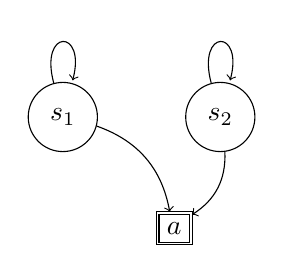
\begin{tikzpicture}[node distance=2cm, auto]
        % States
        \node[state] (s1) {$s_1$};
        \node[state] (s2) [right of=s1] {$s_2$};
        \node[accepting,draw] (a) [below right of=s1] {$a$};

        % Edges
        \path[->] 
            (s1) edge [loop above] ()
            (s1) edge [bend left] (a)
            (s2) edge [loop above] ()
            (s2) edge [bend left] (a);
    \end{tikzpicture}
    \caption{(a)}
    
    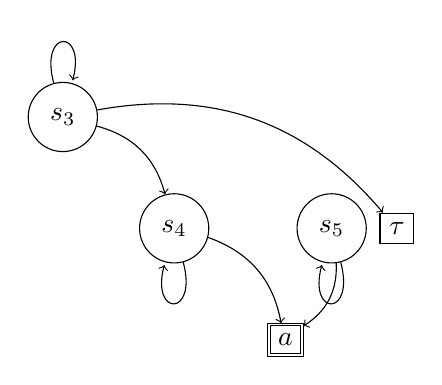
\begin{tikzpicture}[node distance=2cm, auto]
        % States
        \node[state] (s3) {$s_3$};
        \node[state] (s4) [below right of=s3] {$s_4$};
        \node[state] (s5) [right of=s4] {$s_5$};
        \node[accepting,draw] (a) [below right of=s4] {$a$};
        \node[draw] (tau) [above right of=a] {$\tau$};

        % Edges
        \path[->] 
            (s3) edge [loop above] ()
            (s3) edge [bend left] (tau)
            (s3) edge [bend left] (s4)
            (s4) edge [loop below] ()
            (s4) edge [bend left] (a)
            (s5) edge [loop below] ()
            (s5) edge [bend left] (a);
    \end{tikzpicture}
    \caption{(b)}
    
    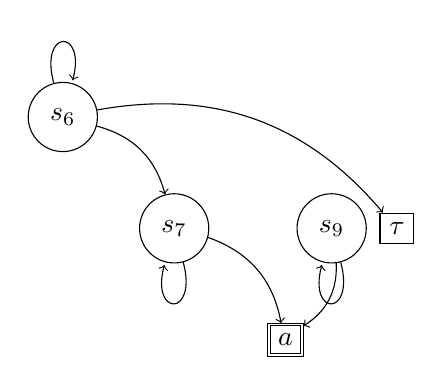
\begin{tikzpicture}[node distance=2cm, auto]
        % States
        \node[state] (s6) {$s_6$};
        \node[state] (s7) [below right of=s6] {$s_7$};
        \node[state] (s9) [right of=s7] {$s_9$};
        \node[accepting,draw] (a) [below right of=s7] {$a$};
        \node[draw] (tau) [above right of=a] {$\tau$};

        % Edges
        \path[->] 
            (s6) edge [loop above] ()
            (s6) edge [bend left] (tau)
            (s6) edge [bend left] (s7)
            (s7) edge [loop below] ()
            (s7) edge [bend left] (a)
            (s9) edge [loop below] ()
            (s9) edge [bend left] (a);
    \end{tikzpicture}
    \caption{(c)}
    \label{fig:sample_318}
\end{figure}

\end{document}